\chapter{Diodes et applications}

	\section{Introduction}
	\begin{wrapfigure}[6]{r}{6.5cm}
	\vspace{-0.5cm}
	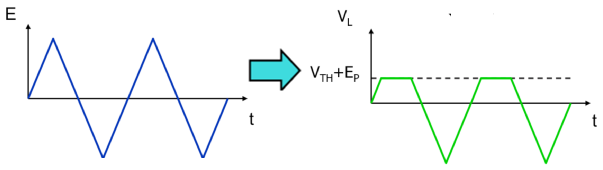
\includegraphics[scale=0.35]{ch5/image1}
	\captionof{figure}{Écrêtage}
	\end{wrapfigure}
	La diode est le plus simple des semi-conducteurs. Leur utilisation principale 
	consiste à redresser une tension : par exemple, changer une tension alternative 
	en une tension intégralement positive. En plus de redresser, on peut également 
	écrêter une tension c'est-à-dire lui imposer une limitation
	
	\section{La diode à jonction PN (idéale)}
	\begin{wrapfigure}[2]{r}{2cm}
	\vspace{-0.5cm}
	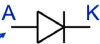
\includegraphics[scale=0.35]{ch5/image2}
	\captionof{figure}{ }
	\end{wrapfigure}
	La diode possède deux bornes : 
	\begin{enumerate}
	\item La borne côté triangle $A$ : l'anode
	\item La borne côté barre $K$ : la cathode
	\end{enumerate}
	La diode possède donc un sens, on ne peut pas switch les deux côtés! Il faut 
	retenir que la cathode émet des électrons, le courant va bien de l'anode à 
	la cathode (les $e^-$ allant en sens inverse). Compte tenu de ces deux bornes, 
	on peut lister une des trois propriétés principales de la diode :
	\begin{wrapfigure}[8]{l}{4cm}
	\vspace{-0.5cm}
	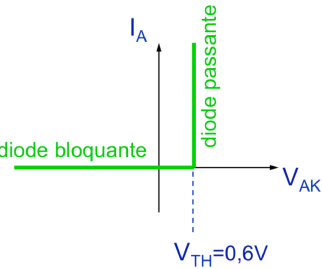
\includegraphics[scale=0.35]{ch5/image3}
	\captionof{figure}{ }
	\end{wrapfigure}
	\begin{enumerate}
	\item Elle n'admet de courant que de $A \rightarrow K$
	\item Elle ne peut que consommer de l'énergie : dipôle passif\footnote{Flèche de 
	tension opposée au courant.}
	\item Elle ne possède que deux états : \textit{passante} (le courant passe) et 
	\textit{bloquante}. C'est salade tout, ou rien.
	\end{enumerate}
	Compte-tenu de cette troisième propriété, la caractéristique $(I,V)$ d'une diode 
	forme un angle droit. Cet angle droit s'observe pour $V_{TH}$, la tension de 
	seuil (souvent 0.6V) qui représente le passage de l'état bloquant à passant.
	
		\subsection{Caractéristique d'une diode idéale}
			\subsubsection{Diode passante}
			La caractéristique nous montre que le courant est positif et que la 
			ddp sur la diode vaut $V_{TH} = 0.6$ V. On peut résumer ceci 
			mathématiquement en
			\begin{equation}
			\left\{\begin{array}{ll}
			V_{AK} &= 0.6\ V\\
			I_A &> 0
			\end{array}\right.
			\end{equation}
			On remarque qu'une diode passant peut être assimilée à une source de 
			tension idéale à valeur $V_{TH}$. En effet, sa caractéristique est une 
			droite verticale et elle impose une ddp mais pas le courant.\\
			Si dans un circuit, les tensions sont bien plus élevée que $V_{TH}$ on 
			peut la remplacer par $V_{TH}=\SI{0}{\volt}$ soit un court-circuit!
			
			\subsubsection{Diode bloquante}
			La caractéristique nous montre que le courant est nul et que la ddp sur 
			la diode est inférieur à 0.6 V. Mathématiquement :
			\begin{equation}
			\left\{\begin{array}{ll}
			V_{AK} &< 0.6\ V\\
			I_A &= 0
			\end{array}\right.
			\end{equation}	
			On peut, avec un raisonnement semblable, associer une diode bloquante à
			un circuit ouvert : il impose un courant nul, mais pas la ddp. Notons 
			cependant que la ddp peut être supérieure à $V_{TH}$ pour le circuit 
			ouvert.\\
			
		Il faut bien garder à l'esprit que la diode est un composant \textbf{non}-
		linéaire, sa caractéristique n'étant pas une droite mais deux demi-droite. 
		En résumé express, la diode (idéale) est un composant semi-conducteur, à deux
		bornes, non symétrique, passif, à deux états et non-linéaire.
		
		
	\section{Résoudre un circuit à diodes}
	\danger Ne surtout pas confondre potentiel (par exemple, sur une des bornes de 
	la diode ($V_A$, $V_L$)) avec une ddp (tension sur la diode ($V_{AK}=V_A-V_K$). 
	C'est bien $V_{AK}$ qui figure sur la caractéristique, ne mélangeons pas tout!
	
		\subsection{Méthode canonique}
			\begin{wrapfigure}[7]{l}{4cm}
	\vspace{-0.5cm}
	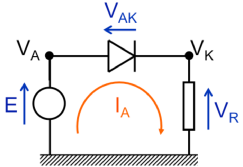
\includegraphics[scale=0.45]{ch5/image4}
	\captionof{figure}{ }
	\end{wrapfigure}
		La première chose à faire est définir les signes des tension et des courants. 
		Il y a alors trois inconnues ($V_{AK}$, $V_R$, $I_A$) et il nous faut autant 
		d'équations :
		\begin{enumerate}
		\item Loi des mailles $E = V_{AK}+V_R$
		\item Loi de la réistance $V_R=RI_A$
		\item Loi de la diode
		\end{enumerate}
		La souci est qu'il n'est pas possible d'écrire la \textit{loi de la diode} 
		en une seule équation à cause de son comportement tout/rien. Pour s'en 
		sortir, il faut suivre un raisonnement par \textbf{hypothèse} : commencer 
		par un \textit{si}.\\
		Cela consiste à : poser une hypothèse, raisonner comme si elle était vraie 
		et vérifier ensuite si le résultat est compatible avec l'hypothèse.
		
		\newpage
		\begin{wrapfigure}[10]{r}{7cm}
%	\vspace{-0.5cm}
	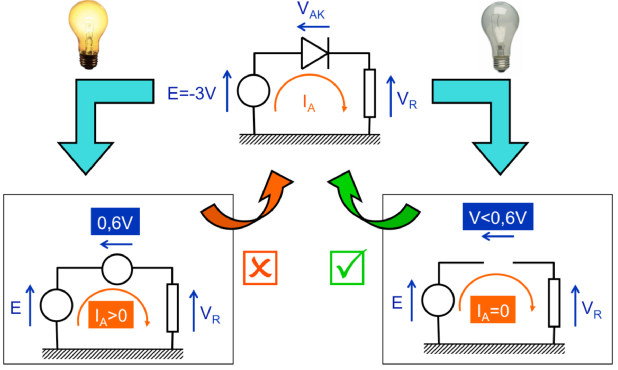
\includegraphics[scale=0.35]{ch5/image5}
	\captionof{figure}{ }
	\end{wrapfigure}
		Dans notre cas, supposons que la diode est passante : je peux la remplacer 
		par une source de tension et résoudre le circuit\footnote{Conseil : redessiner 
		le circuit}. Comme par hypothèse $V_{AK}=0.6\ V$, si $I_A>0$ c'est en principe 
		bon (vérifiez quand même l'autre cas!). On aurait pu également prendre la 
		seconde hypothèse : remplacer la diode par un circuit ouvert. Si $V_{AK}<0.6\ V$
		alors ce serait bon.\\
		On remarque que le test de l'hypothèse se fait avec l’inégalité. Pour des 
		exemples de calcul, voir p.~20--23.\\
		
		Une résolution graphique est également possible : il faut dessiner, sur le 
		même graphique, la caractéristique de la diode et celle du circuit extérieur. 
		En fonction du point d'intersection, on peut déterminer l'état de la diode. 
		Ceci n'est faisable que pour des circuits extérieurs simples !\\
		\danger En synthèse, il faut bien raisonner par hypothèses et surtout ne \textbf{pas} 
		utiliser la superposition!
			
			
	\section{Diodes et polarisation}
	Polariser un élément, c'est l'amener dans une certaine situation électrique via un 
	circuit extérieur (souvent avec des sources continues). C'est intéressant pour 
	la diode, car cela permet de contrôler son état.\\
	
	Avant tout, un peu de vocabulaire : une diode est en polarisation \textit{directe }
	ou \textit{indirecte} suivant le signe de $V_{AK}$. Si cette ddp est positive, la 
	polarisation est dite \textit{directe} et \textit{inverse} dans le cas contraire.
	
		\subsection{Rendre une diode bloquante}
		Il suffit de faire quelque chose que toi, oui toi, fait très bien : rien. En 
		effet, si la diode n'est connectée à rien elle est spontanément bloquante. 
		Elle reste bloquante tant qu'on lui impose une tension inférieur à 0.6 V.
			
		\subsection{Rendre une diode passante}
		\begin{wrapfigure}[8]{r}{7cm}
		\vspace{-0.5cm}
		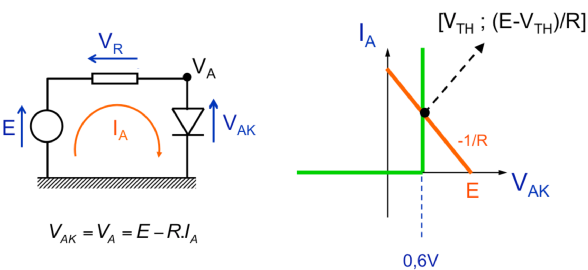
\includegraphics[scale=0.35]{ch5/image6}
		\captionof{figure}{ }
		\end{wrapfigure}
		Pour se faire, il ne faut \textbf{surtout pas} lui appliquer directement une 
		fem ($\geq 0.6\ V$). Deux cas possibles :
		\begin{enumerate}
		\item Si la fem vaut $V_{TH}$, les caractéristiques se superposent et aucun 
		point de fonctionnement n'est défini : $I_A$ indéterminé.
		\item Si la fem est supérieure à $V_{TH}$ les caractéristiques ne se croisent 
		pas : $I_A = \infty$.
		\end{enumerate}
		Pour régler le problème, il faut utiliser une \textit{résistance de limitation 
		de courant} : on lui tape une résistance en série. Cela va incliner la 
		caractéristique du circuit extérieur et donner lieu à un point d'intersection 
		donnant lieu à un courant non-infini : $I = (E-V_{TH})/R$. Dans la pratique, 
		le dimensionnement se fait via $R$. Il est également possible de rendre une 
		diode passante avec une source de courant connectée dans le \textbf{bon} sens.
		
		\newpage
		
	\section{Principaux circuits à diodes}
		\subsection{Redresseur simple alternance}
		Il s'agit du circuit à diode le plus simple : une source de tension, une iode 
		et une résistance. La résolution du circuit donne lieu (si la source de tension 
		est un paramètre) à deux cas :
		\begin{itemize}
		\item Diode passante si $E > V_{TH}$
		\item Diode bloquante si si $E < V_{TH}$
		\end{itemize}
		Si l'on applique une tension alternative, seules les valeurs positives de $E$ 
		(à $V_{TH}$ près) passeront et les autres seront bloquées.
		\begin{center}
		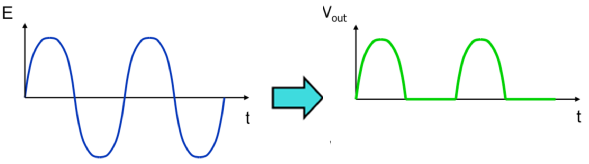
\includegraphics[scale=0.45]{ch5/image7}
		\captionof{figure}{ }
		\end{center}
		
		\subsection{Sélecteur de maximum/minimum}
		\begin{wrapfigure}[8]{r}{3cm}
		\vspace{-0.5cm}
		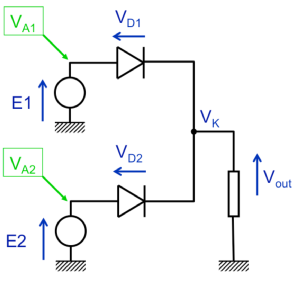
\includegraphics[scale=0.35]{ch5/image11}
		\captionof{figure}{ }
		\end{wrapfigure}
		Il faut appliquer la méthode vue, pour quatre cas possibles : chacune des 
		deux diodes peut être dans les deux états. Supposons $E_1>E_2>0$ et 
		calculons $V_{out}$. Soit $D_1$, $D_2$, nos deux diodes.\\
		Si $D_1$ est passante, $V_K = E_1-0.6\ V$.
		\begin{itemize}
		\item[$\bullet$] Si $D_2$ est passante, $V_K = E_2-0.6\ V$ ce qui est 
		impossible : les deux ne peuvent pas être passantes.
		\item[$\bullet$] Si $D_2$ est bloquante, on peut la modéliser par un 
		circuit ouvert : le courant dans $D_1$ est positif, elle peut donc être 
		passante. La ddp sur $D_2$ vaut $V_{A2}-V_K < 0.6\ V$ c'est bon !
		\end{itemize}
		La situation $D_1$ passante et $D_2$ bloquante est bonne. On peut faire 
		un même raisonnement dans le cas inverse pour en venir à la conclusion 
		que $V_{out} = \max(E_1,E_2)$.
		
		\subsection{Redresseur double alternance}
			\subsubsection{Schéma à deux diodes}
			Il transforme \textit{toutes} les alternances (positives et négatives) 
			de la tension d'entrée en alternances positives de la tension de sortie. 
			On peut le réaliser avec deux diodes, mais il faut alors deux sources 
			de courant identiques.
			\begin{center}
			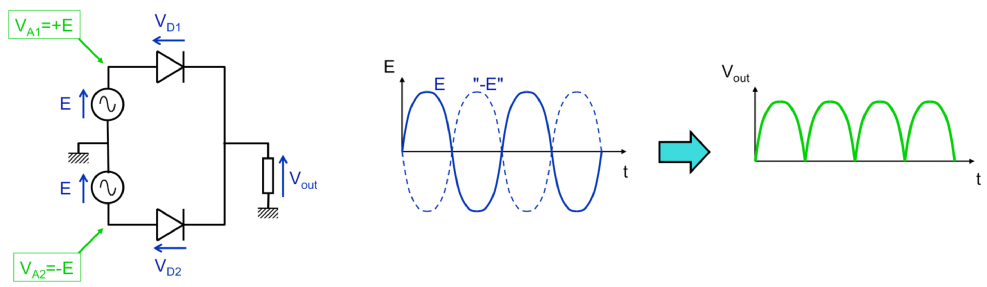
\includegraphics[scale=0.45]{ch5/image8}
			\captionof{figure}{ }
			\end{center}
			On peut raisonner de façon semblable au secteur vu précédemment ou 
			utiliser un raisonnement alternatif :
			\begin{itemize}
			\item[$\bullet$] L'anode de $D_1$ est au potentiel $V_{A1} = 0+E$ 
			(sinusoïdale continue)(0 vient de la masse)
			\item[$\bullet$] L'anode de $D_2$ est au potentiel $V_{A_2} = 0-E=-E$ 
			(sinusoïdale discontinue)(sens de la flèche cause le -)
			\end{itemize}
			Il s'agit en fait d'un sélecteur de maximum avec deux sources opposées 
			l'une de l'autre : seule l'alternance positive est sélectionnée.
			
			\subsubsection{Pont à quatre diodes}
			Il est possible de faire de même avec une seule source, mais cela 
			nécessite quatre diodes.
			\begin{center}
			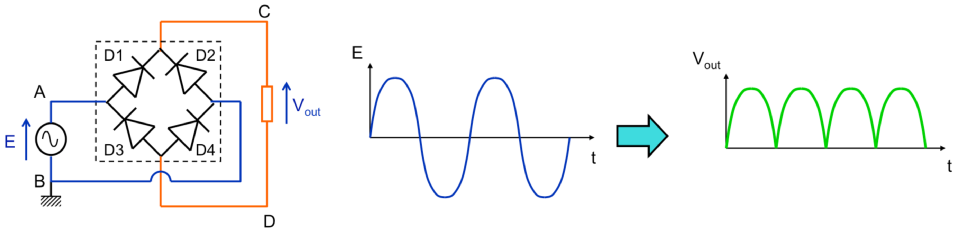
\includegraphics[scale=0.45]{ch5/image9}
			\captionof{figure}{Remarquez le "sens" des diodes (pour sélectionner le 
			minimum}
			\end{center}		
			En se basant sur les propriétés du sélecteur, on peut dire que :
			\begin{multicols}{2}
			\begin{enumerate}
			\item Si $E>0 \rightarrow V_A>V_B$
				\begin{itemize}
				\item[$\bullet$] $D_1/D_2$ prends le max, c'est à dire $V_C=V_A$.
				\item[$\bullet$] $D_3/D_4$ prends le min, c'est à dire $V_D=V_B$.
				\item[$\bullet$] $V_{out} = V-C-V_D = V_A-V_B=E$
				\end{itemize}\ \\
				
			\item Si $E<0 \rightarrow V_A<V_B$
				\begin{itemize}
				\item[$\bullet$] $D_1/D_2$ prends le max, c'est à dire $V_C=V_B$.
				\item[$\bullet$] $D_3/D_4$ prends le min, c'est à dire $V_D=V_A$.
				\item[$\bullet$] $V_{out} = V-C-V_D = V_B-V_A=-E >0$
				\end{itemize}			
			\end{enumerate}
			\end{multicols}
		
		\subsection{Limiteur de tension (écrêteur)}
		Ceci est fortement utiliser pour protéger une composante. Pour être rigoureux, 
		il faudrait faire un raisonnement par hypothèses. On peut gagner du temps en 
		remarquant que si on "oublie" la diode, on trouve un diviseur résistif.
					\begin{center}
			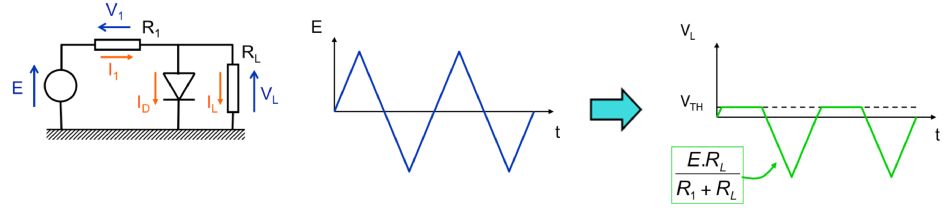
\includegraphics[scale=0.45]{ch5/image10}
			\captionof{figure}{ }
			\end{center}		
			
		Si la diode est passante $V_L=V_{AK}=0.6\ V$.
		\begin{itemize}
		\item[$\bullet$] Le courant dans $R_L$ vaut $I_L = 0.6/R_L$
		\item[$\bullet$] Le courant dans $R_1$ vaut $I_1 = (E-0.6)/R_1$		
		\item[$\bullet$] Le courant dans $D$ est la différence entre les deux : $I_D 
		= I_1-I_L$.
		\item[$\bullet$] $I_D > 0 \Rightarrow E.R_L(R_1+R_L)>V_{TH}$
		\end{itemize}
		Si la diode est bloquante 
		\begin{itemize}
		\item[$\bullet$] Diviseur résistif  $V_{out} = E.R_L(R_1+R_L)$
		\item[$\bullet$] Valable que si la ddp sur la diode $<V_{TH}$ : 
		$E.R_L(R_1+R_L)<V_{TH}$
		\end{itemize}				
		On peut vérifier (ça se sent directement intuitivement, la tension aux bornes 
		d'une diode ne pouvant dépasser $V_{TH}$) que la tension sur 
		la charge ($R_L$) ne dépasse jamais $V_{TH}$.
		
		
		\subsection{Ecrêteur polarisé}
		Le montage précédent ne permet que de protéger à hauteur de $V_{TH}$. Si 
		on veut une autre valeur, il sufit de rajouter une source de tension continue 
		en série avec la diode et le tour est joué!
			
		
		\subsection{Détecteur de crête}
			
			
			
			
			
			
			
			
			
			
			
			
			
			
			
			
			
			
			
			
